\documentclass[a4paper]{article}
\usepackage[14pt]{extsizes} % для того чтобы задать нестандартный 14-ый размер шрифта
\usepackage{amsmath}
\usepackage[unicode, pdftex]{hyperref}
\usepackage[usenames]{color}
\usepackage[warn]{mathtext}
\usepackage[T2A]{fontenc}
\usepackage[utf8]{inputenc}
\usepackage[english, russian]{babel}
\usepackage{amsfonts}
\usepackage[left=20mm, top=15mm, right=15mm, bottom=15mm, nohead, footskip=10mm]{geometry} % настройки полей документа
\usepackage{graphicx}
\usepackage{wrapfig}
\usepackage{placeins}
\usepackage{float}
\usepackage{ucs}
\begin{document}
\author{Горяной Егор}
\date{28 мая 2022}
\title{Дифракция на CD-диске}
\maketitle


\section{Теоретическая часть}
{Для того, чтобы записывать информацию на CD-диск, в нём делают специальный углубления --- питы. Каждый пит имеет примерно 100 нм в глубину и 500 нм в ширину. Длина пита варьируется от 850 нм до 3,5 мкм. Шаг дорожек в спирали составляет 1,6 мкм. Питы рассеивают или поглощают падающий на них свет, а подложка — отражает. Поэтому записанный компакт-диск — пример отражательной дифракционной решётки с периодом порядка нескольких микрон.}
\begin{figure}[H]
    \centering
    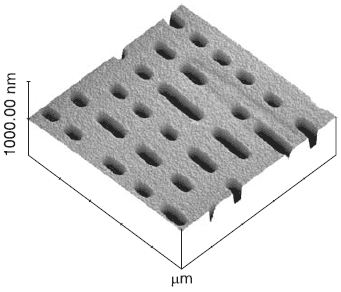
\includegraphics[scale=1]{cd_disk.png}
    \caption{CD-диск под микросопом}
\end{figure}
Уравнение решётки в случае нормального падения света:
\begin{equation}\label{eq1}
d\sin\theta_m=m\lambda
\end{equation}
Пусть свет падает нормально в точку, находящуюся на расстоянии $R$ от центра диска. Тогда расстоянию $d$ соответствует какой-то угол $\Delta\varphi$.\\
\\
При этом имеем равенство: $\Delta\varphi=\displaystyle\frac{d}{R}$.\\
\\
При этом сумма всех углов даст нам угловой размер окружности, то есть $2\pi$:
\begin{equation}\label{eq2}
\displaystyle\sum\limits_{i=1}^{N}\Delta\varphi_i =2\pi
\end{equation}
\\
С другой стороны:
\begin{equation}\label{eq3}
\sum\limits_{i=1}^{N}\Delta\varphi_i=\sum\limits_{i=1}^{N}\displaystyle\frac{d}{R} = N \displaystyle \frac {d}{R}
\end{equation}
\\
Приравнивая (2) и (3), получим:
\begin{equation}\label{eq4}
N=\displaystyle\frac{2\pi R}{d}
\end{equation}
\\
При этом разрешающая способность решётки:
\begin{equation}\label{eq5}
R=mN=\displaystyle\frac{\lambda}{\delta\lambda}
\end{equation}
\\
Подставим $m=1,$ (1) и (4) в (5) и выразим $\delta\lambda$:
\begin{equation}\label{eq6}
\delta\lambda=\displaystyle\frac{\lambda^2}{2\pi R\sin\theta_1}
\end{equation}
\\
\pagebreak
\section{Практическая часть}\\
Соберём установку и измерим расстояния:\\
\begin{figure}[H]
    \centering
    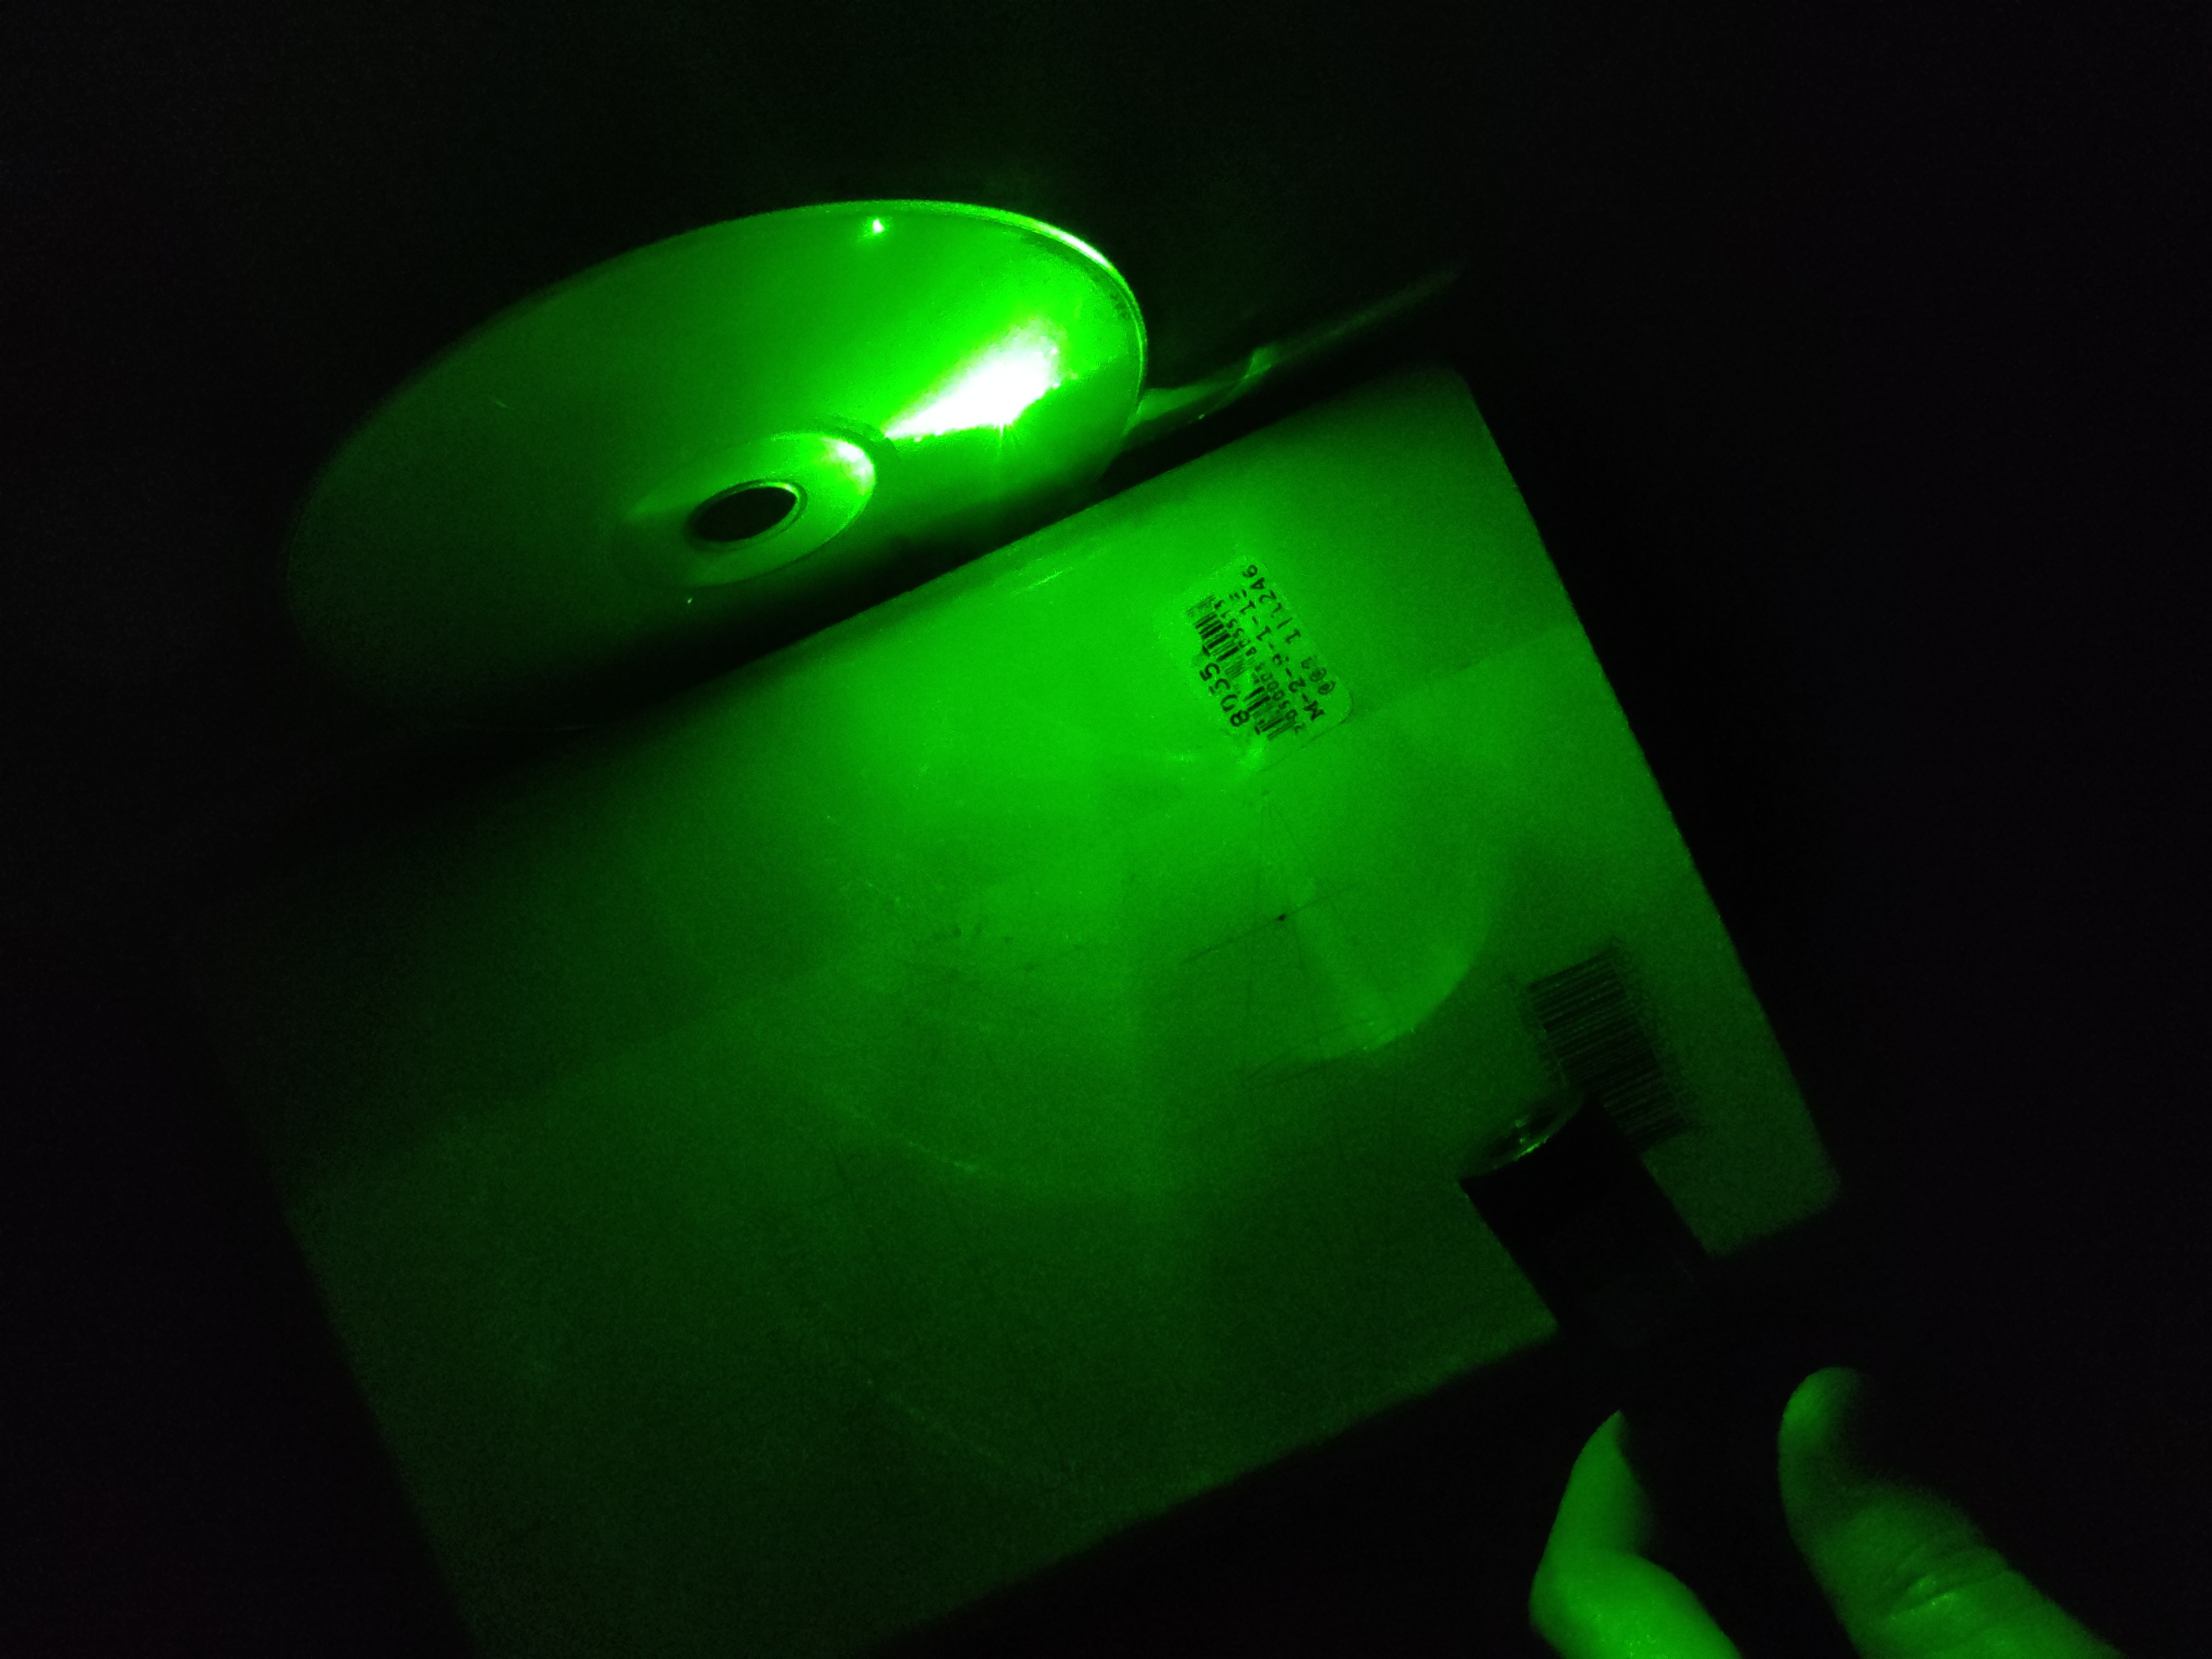
\includegraphics[scale=0.1]{ust.jpg}
    \caption{установка}
\end{figure}
\begin{figure}[H]
    \centering
    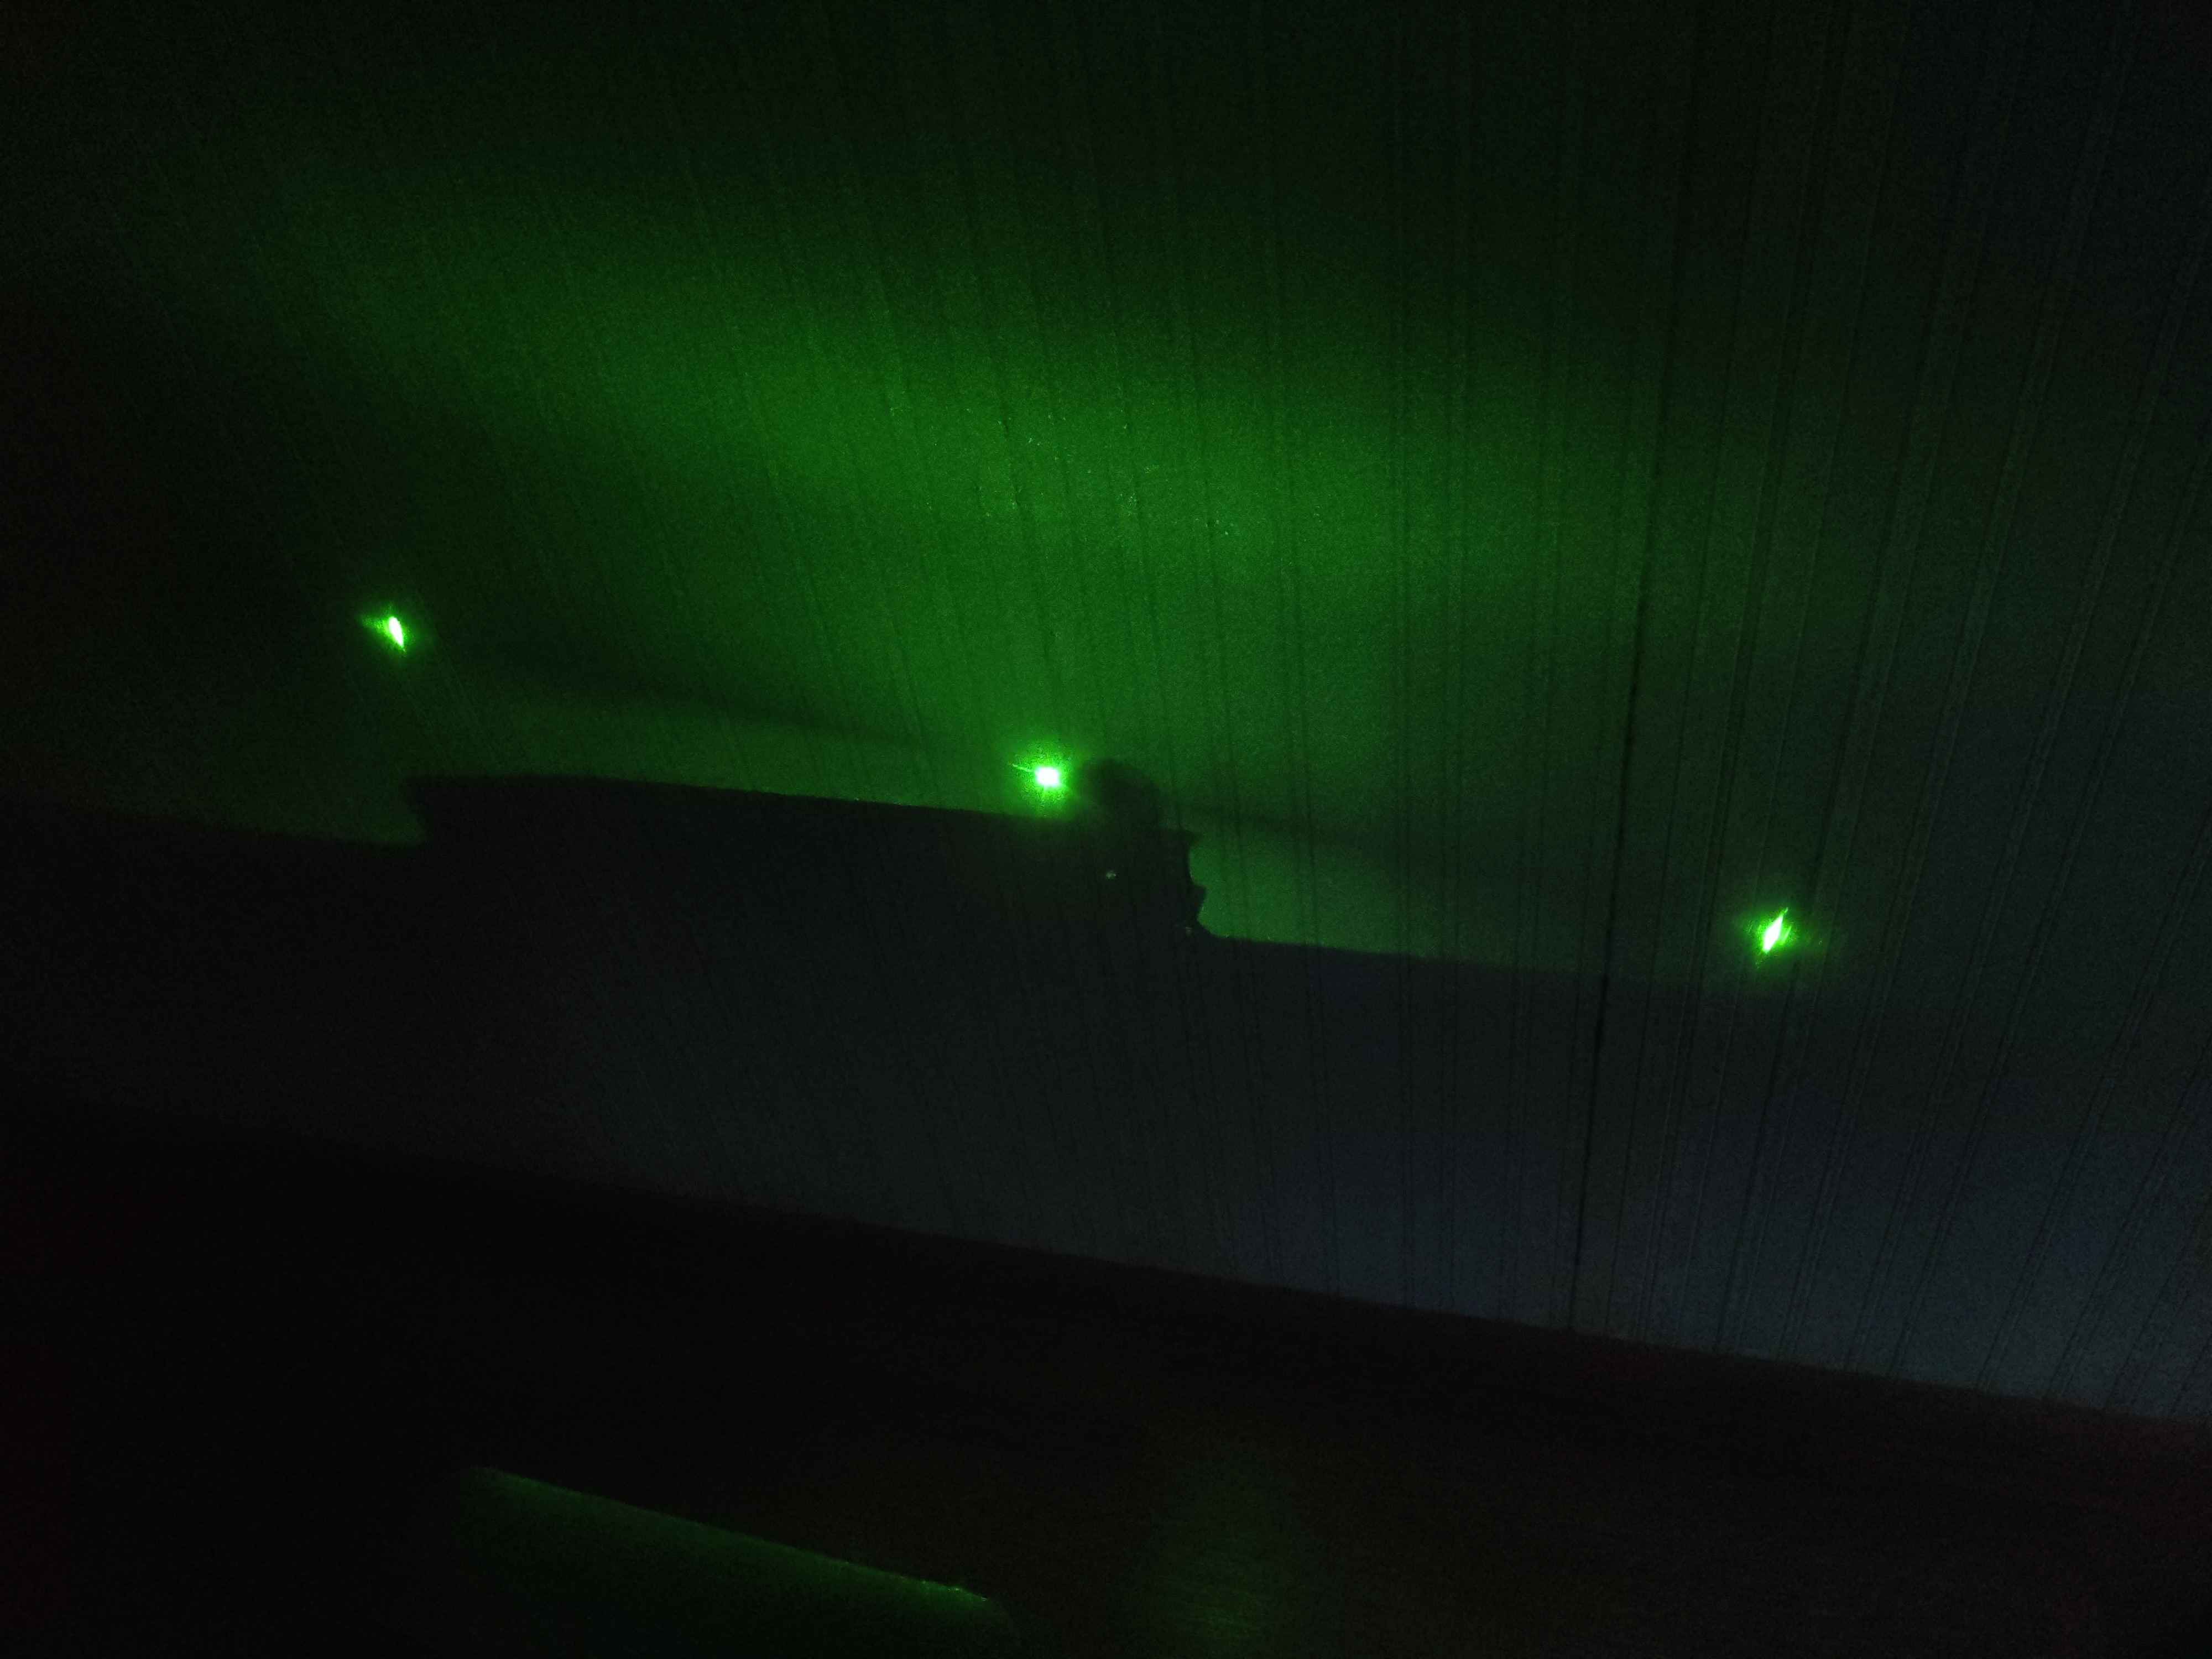
\includegraphics[scale=0.1]{diffrac.jpg}
    \caption{дифракционная картина}
\end{figure}
\\
$L=1.11$ м, $l_1=43$ см, $l_2=1.16$ м, $R=2.5$ см, где $L$ --- расстояние от дифракционной решетки до экрана(стены),
$l_1,~l_2$ --- расстояния от нулевого максимума дифракционной картины до 1-го и 2-го соответственно, $R$ --- расстояние
от центра диска до точки, в которую приходит луч лазера.\\
\\
$\sin\theta_{1,2}=\displaystyle\frac{l_{1,2}}{\sqrt{L^2+l_{1,2}^2}}$. В таком случае получим, что:\\
\\
$\sin\theta_1\approx0.36,~\sin\theta_2\approx0.72$\\\
\\
Зелёный свет соответствует длине волны $\lambda=532$ нм. Тогда, подставляя $\lambda=532$ нм в (1), получим следующие результаты:
\\
\\
\begin{tabular}{lllll}
\cline{1-3}
\multicolumn{1}{|l|}{}  & \multicolumn{1}{l|}{$m=1$}   & \multicolumn{1}{l|}{$m=2$}   &  &  \\ \cline{1-3}
\multicolumn{1}{|l|}{$d$, мкм} & \multicolumn{1}{l|}{1.473} & \multicolumn{1}{l|}{1.477} &  &  \\ \cline{1-3}
                        &                            &                            &  &  \\
                        &                            &                            &  &
\end{tabular}
\\
Максимальному порядку соответствует $\sin\theta_{max}=1$. Подствавляя это в (1) и усредняя $d$ по двум измерениям,
получим, что $m_{max}=\displaystyle\frac{d_{mean}}{\lambda}\approx2.8<3$. Это объясняет,
почему мы не видим уже 3-го максимума.\\
Найдём теперь  спектральное разрешение $\delta\lambda$ по ф-ле (6):
\begin{equation}\label{eq7}
\delta\lambda=\displaystyle\frac{\lambda^2}{2\pi R\sin\theta_1}\approx5~пкм
\end{equation}
Тогда разрешающая способность решётки в первом порядке дифракции равна:
\begin{equation}\label{eq8}
R=\displaystyle\frac{\lambda}{\delta\lambda}\approx106400
\end{equation}
Оценим погрешности для $\delta\lambda,~R$:
    $$ \delta\lambda=5\pm 0.1~пкм$$
    $$ R=106400\pm2128 $$
\end{document}


